\documentclass[11pt]{article}
\usepackage{latexsym}
\usepackage{amsmath}
\usepackage{amssymb}
\usepackage{amsthm}
\usepackage{epsfig}
\usepackage[tight]{subfigure}

\usepackage{amsmath}

\DeclareMathOperator*{\minimize}{min}
\DeclareMathOperator*{\maximize}{max}

\DeclareMathOperator*{\argmax}{argmax} % thin space, limits underneath in displays

\usepackage{algorithm}
 %on linux you may need to run sudo apt-get install texlive-full to install algorithm.sys
\usepackage{algorithmic}

\usepackage{verbatim}

\newcommand{\handout}[5]{
  \noindent
  \begin{center}
  \framebox{
    \vbox{
      \hbox to 5.78in { {#1} \hfill #2 }
      \vspace{4mm}
      \hbox to 5.78in { {\Large \hfill #5  \hfill} }
      \vspace{2mm}
      \hbox to 5.78in { {\em #3 \hfill #4} }
    }
  }
  \end{center}
  \vspace*{4mm}
}

\newcommand{\lecture}[5]{\handout{#1}{#2}{#3}{#4}{#5}}
\newcommand{\collision}[0]{\mathrm{collision}}
\newcommand{\nocollision}[0]{\overline{\collision}}

\newcommand*{\QED}{\hfill\ensuremath{\square}}

\newtheorem{theorem}{Theorem}
\newtheorem{corollary}[theorem]{Corollary}
\newtheorem{lemma}[theorem]{Lemma}
\newtheorem{observation}[theorem]{Observation}
\newtheorem{proposition}[theorem]{Proposition}
\newtheorem{definition}[theorem]{Definition}
\newtheorem{claim}[theorem]{Claim}
\newtheorem{fact}[theorem]{Fact}
\newtheorem{assumption}[theorem]{Assumption}
\newtheorem{note}[theorem]{Note}

% 1-inch margins, from fullpage.sty by H.Partl, Version 2, Dec. 15, 1988.
\topmargin 0pt
\advance \topmargin by -\headheight
\advance \topmargin by -\headsep
\textheight 8.9in
\oddsidemargin 0pt
\evensidemargin \oddsidemargin
\marginparwidth 0.5in
\textwidth 6.5in

\parindent 0in
\parskip 1.5ex
%\renewcommand{\baselinestretch}{1.25}

\begin{document}

\lecture{Statistical Techniques in Robotics (16-831, S22)}{Lecture \#05
  (Wednesday, February 2)}{Lecturer: Kris Kitani}{Scribes: John Harrington, Russell Wong (Group 1)}{Online Linear Classification}

\section{Review}



%This section serves as a review of the previous lecture and any other context required to frame the content of the current lecture. 

%You may format the scribes in any way you like, aside from changing font style, size and page format. Please use subsections and paragraphs to increase the readability of your notes.

%Length requirement 1-2 pages.

In the previous lecture, we had discussed further examples of \textbf{PWEA} (Prediction with Expert Advice) as well as diving into the performance and guarantees of such algorithms. We explored two additional algorithms to address the PWEA problem, the Weighted Majority Algorithm (\textbf{WMA}) and the Randomized Weighted Majority Algorithm (\textbf{RWMA}) \cite{hoi2018online}.
        
\subsection{Weighted Majority Algorithm}

Unlike other PWEA methods that had been explored previously, the Weighted Majority Algorithm does not assume realizability, and permits the best hypothesis to make mistakes. Rather than maintaining a version space of hypotheses and removing the ones that make mistakes, the WMA maintains an $N$-dimensional weight vector, $\boldsymbol{w}^{(t)}$. This weight vector is used to inform the learner's predictions $\hat{y}^{(t)}$ by taking the sign of the dot product of $\boldsymbol{w}^{(t)}$ with the observation $\boldsymbol{x}^{(t)}$. This effectively relatively weights the individual features of $\boldsymbol{x}^{(t)}$ and their contributions to the prediction. During the previous lecture it was also noted that, with this new prediction rule, the hypothesis class is the set of all positively weighted linear classifiers (here we assume $\boldsymbol{w}\in(0,1]^N$). The concept of linear classification will be further explored and defined as a part of this lecture.

The weight vector is then updated according to a penalty parameter $\eta$, which dictates how individual elements of the weight vector should be penalized, depending on whether a feature/expert has made a mistake. These ideas of maintaining a weight vector rather than a version space, and updating this weight vector according to mistakes made, are built upon in this lecture as well.

Since we are no longer maintaining a version space, a new potential function must also defined. In the previous lecture we used $\Phi^{(t)} = \sum_{n=1}^{N}w_n^{(t)}$, which is somewhat analogous to the size of the version space used previously as a potential function. We will see that a similar potential function will be used in bounds derivation during this lecture, only taking the sum of the weights \textbf{squared} instead.

The following relative mistake bound and regret bound were derived for the WMA:

$$M^{(T)} \leq 2(1+\eta)m_n^{(T)}+\frac{2\ln N}{\eta}$$
\begin{equation}
R(h_n)\leq m_n^{(T)}+2\eta m_n^{(T)} + \frac{2\ln N}{\eta}
\label{eq:wma-regret}    
\end{equation}

Where $M^{(T)}$ is the number of mistakes made by the learner up to time $T$, $m_n^{(T)}$ is the number of mistakes made by the $n^{\text{th}}$ expert up to time $T$, and $R(h_n)$ is the regret relative to hypothesis $h_n$ \cite{shalev-shwartz} .

\subsection{Randomized Weighted Majority Algorithm}

The RWMA builds upon the WMA by introducing randomization. Specifically, instead of directly using $\boldsymbol{w}^{(t)}$ to relatively weight the features of $\boldsymbol{x}^{(t)}$, a selector function $h$ is sampled from a multinomial distribution with probability relative to the weights. The prediction $\hat{y}^{(t)}$ is then computed from this selector function as $h(\boldsymbol{x}^{(t)})$. Using the same potential function of $\Phi^{(t)} = \sum_{n=1}^{N}w_n^{(t)}$, the following relative mistake bound and regret bound were derived:

$$\mathbb{E}[M^{(T)}]\leq (1+\eta)m_n^{(T)}+\frac{\ln N}{\eta}$$
\begin{equation}
\mathbb{E}[R]\leq \eta m_n^{(T)} + \frac{\ln N}{\eta}
\label{eq:rwma-regret}    
\end{equation}

Here, $\mathbb{E}$ denotes expectation. Furthermore, as shown previously, $M^{(T)}$ is the number of mistakes made by the learner up to time $T$, $m_n^{(T)}$ is the number of mistakes made by the $n^{\text{th}}$ expert up to time $T$, $N$  is the number of elements in $\boldsymbol{w}^{(t)}$, $\eta$ is the penalty parameter, and $R$ is regret.  

\subsection{Analyses of Regret Bounds}

In the previous lecture, it was noted that by carefully selecting $\eta$, one could make these algorithms bounded or no-regret: particularly, if $\eta$ is selected to be time-varying \cite{orabona}.

First, recall that a no-regret algorithm requires the regret bound to be sub-linear in $T$. Additionally, note that $m_n^{(T)}$ grows linearly on the order of $O(T)$, and $\ln N$ is constant with time, on the order of $O(1)$. For the RWMA, it is possible to achieve no-regret by selecting $\eta$ to be time-varying, with $\eta$ on the order of $O\left(\frac{1}{\sqrt{T}}\right)$. In this case, the first term in Equation (\ref{eq:rwma-regret}) is $O\left(\frac{1}{\sqrt{T}}\right) \times O(T) = O(\sqrt{T})$, and the second term is $O(1) \div {O\left(\frac{1}{\sqrt{T}}\right)} = O(\sqrt{T})$. Hence, the overall regret bound is sub-linear in $T$ and therefore RWMA can be considered to be a no-regret algorithm (with this appropriate selection of $\eta$).

On the other hand, the WMA cannot be made into a no-regret algorithm. The regret bound for the WMA, as indicated in Equation (\ref{eq:wma-regret}), contains a $m_n^{(T)}$ term which is on the order of $O(T)$. Even if $\eta$ is selected to be time-adaptive, this will only impact the asymptotic behavior of the last two terms, and the first term $m_n^{(T)}$ will be unaffected. For this reason, the regret bound can be made $O(T)$ at best, meaning that the WMA is a bounded-regret algorithm, but not no-regret. This further reinforces the reasoning behind adding randomization to improve the expected upper bound of regret, as seen in previous lectures.

\section{Online Linear Classification}\label{section:linear_classification}

The problem of online linear classification is concerned with correctly mapping input features to correct output classifications. For example, if we are trying to determine whether a orange is of high or low quality, this would be a binary linear classification problem, where the input features would be any information used to determine the quality of the orange (size, color, symmetry, markings, etc.). Formally, the goal of online linear classification is to learn a mapping from $\{\boldsymbol{x} \rightarrow\ y\}$, where $\boldsymbol{x} \in \mathcal{X}$ is a vector of input features and $y \in \mathcal{Y}$ is the classification.

We refer to this problem as ``\textbf{online}" in the sense that the classifier continuously receives new inputs at each time step and must update its parameters accordingly, as opposed to being pre-trained on a static data set of examples before deployment. We refer to the classifier as ``\textbf{linear}" to indicate the type of decision boundary that this classifier will learn. Specifically, a linear classifier would learn a decision boundary defined by an $N$-dimensional hyperplane:

$$ \boldsymbol{w} \cdot \boldsymbol{x} $$

Where $ \boldsymbol{w} \in \mathbb{R}^N$ represents the hyperplane parameters and $\boldsymbol{x} \in \mathbb{R}_+^N$ is the feature vector.

(Note that here we define $\boldsymbol{x}$ to consist of only positive-valued numbers, though this does not always have to be the case; e.g. we could have $\boldsymbol{x}\in\mathbb{R}^N$).

In a binary classification problem, we consider the true label $y$ to have one of two possible values, e.g. $y\in \{1,-1\}$. The goal of a binary linear classifier is to learn hyperplane parameters $\boldsymbol{w}$ such that positive examples $\{\boldsymbol{x}_+ \rightarrow y=1\}$ are above the hyperplane, and negative examples $\{\boldsymbol{x}_- \rightarrow y = -1\}$ are below the hyperplane, by some threshold $N$:

$$\boldsymbol{w} \cdot \boldsymbol{x}_{+} \geq N $$

$$\boldsymbol{w} \cdot \boldsymbol{x}_{-} < N $$

This leads to the following prediction rule:

$$\hat{y} = \text{sign}(\boldsymbol{w} \cdot \boldsymbol{x} - N) $$


In the context of online learning, we will discuss two algorithms that will learn online linear classifiers through additive updates (the Perceptron algorithm), and multiplicative updates (the Winnow Algorithm).

\section{Perceptron Algorithm}\label{section:perceptron}

\subsection{Overview}

The \textbf{perceptron} was first introduced as a mathematical model of memory units in biological systems, or neurons  \cite{rosenblatt}. The precise architecture of a perceptron is depicted in Figure \ref{fig:perceptron}. The input to a perceptron is a feature vector $\boldsymbol{x} = \{x_1, x_2,\dots, x_N\}$, with each feature being multiplied by a corresponding weight in the weight vector $\boldsymbol{w}=\{w_1, w_2,\dots, w_N\}$. The weighted features are then summed, along with a constant bias term $b$, and this sum is passed through an activation function $f$ to generate some output $y$. In short, the perceptron models the following input-output relationship:

$$y = f(\boldsymbol{w}\cdot\boldsymbol{x}+b)$$

\begin{figure}[H]
    \centering
    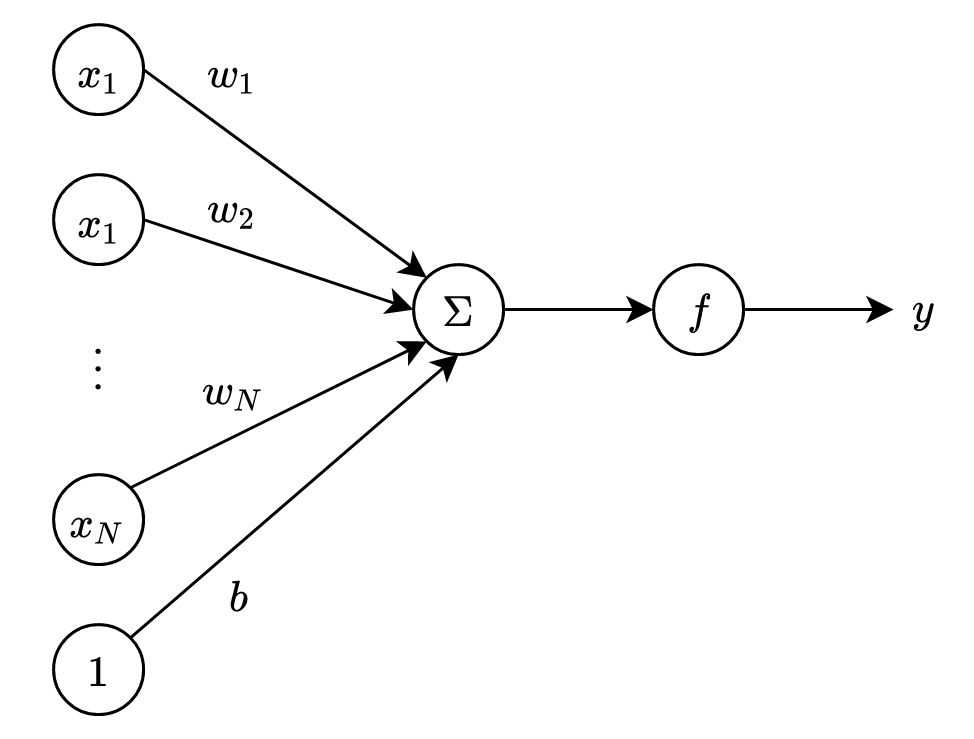
\includegraphics[width=10cm]{Perceptron Diagram.png}
    \caption{Perceptron Model}
    \label{fig:perceptron}
\end{figure}


The \textbf{Perceptron Algorithm} utilizes this model to make predictions in the context of online learning. In a linear classification problem, the activation function $f$ is set to the sign function. The online learner would then be making predictions according to:

$$\hat{y} = \text{sign}(\boldsymbol{w}\cdot\boldsymbol{x}+b)$$

The goal of the online learner is to learn the parameters $\boldsymbol{w}$ and $b$ in order to compute predictions $\hat{y}$ that match the true labels $y$.

Let $\boldsymbol{w}^{(t)}$ be the weights at time step $t$, $T$ be the maximum time step (assumed to be infinity), $\boldsymbol{x}^{(t)}$ be the input or observation at time step $t$, and $y^{(t)}$ be the true label at time step $t$.

The Perceptron Algorithm is presented in Algorithm \ref{algo:perceptron}:

\begin{algorithm}[H]
\caption{Perceptron Algorithm}
\label{algo:perceptron}
\begin{algorithmic}[1]
\STATE $\boldsymbol{w}^{(0)} \xleftarrow{} 0 $  \hfill $\triangleright$ Initialize weights
\FOR{$t=1,\;\dots,\;T$}
\STATE \textsc{Receive} ($\boldsymbol{x}^{(t)} \in \mathbb{R}^N$) \hfill $\triangleright$ Receive observations
\STATE $\hat{y}^{(t)} = \text{sign} \left( \langle \boldsymbol{w}^{(t-1)}, \boldsymbol{x}^{(t)} \rangle \right)$ \hfill $\triangleright$ Make prediction based on observations
\STATE \textsc{Receive} ($y^{(t)}\in \{1,-1\}$) \hfill $\triangleright$ Receive true label
\STATE $\boldsymbol{w}^{(t)} = \boldsymbol{w}^{(t-1)} + y^{(t)} \cdot \boldsymbol{x}^{(t)} \cdot \boldsymbol{1}[y^{(t)}\neq\hat{y}^{(t)}] $ \hfill $\triangleright$ Update weights
\ENDFOR
\end{algorithmic}
\end{algorithm}

Line 4 makes a prediction $\hat{y}^{(t)}$ by passing the input $\boldsymbol{x}^{(t)}$ through the perceptron model. Note that there has been a slight change in notation, as the bias term $b$ is no longer explicitly mentioned. Here it is implied that $b$ is appended as an element of the weight vector, and there is a corresponding element appended to $\boldsymbol{x}^{(t)}$ that is set to $1$. Therefore the summation previously represented by $\boldsymbol{w}\cdot\boldsymbol{x}+b$ can now be represented by the single dot product in Line 4, $\langle \boldsymbol{w}^{(t-1)}, \boldsymbol{x}^{(t)} \rangle$.

It is noted that this algorithm can be computed quickly, based on the efficient additive update in Line 7. However, the classifier does not consider the margin of the data when determining an optimal strategy, meaning that it does not attempt to maximize the margin. Further, since the algorithm does not work with non-separable data, no optimal classifier can be learned for data with overlapping classes. For that reason, the perceptron algorithm \textbf{assumes realizability}, such that there exists a perfect classifier that makes no mistakes. This is equivalent to saying that we assume the data is \textbf{linearly separable}. The perceptron algorithm has been extended in further works to account for these limitations \cite{shalev-shwartz--singer}. 

\subsection{Mistake Bounds Derivation}

\theorem{Let $M^{(T)}$ be the total number of mistakes made by a learner using the Perceptron Algorithm, $R$ be an upper bound on the norm of observations $\boldsymbol{x}^{(t)}$, $\gamma$ be the margin of separability, and $\boldsymbol{w}^*$ be the weights associated with a realizable perfect linear classifier. The number of mistakes $M^{(T)}$ is bounded by:

$$M^{(T)} \le \frac{R^2}{\gamma^2}$$

Where:

\begin{equation}
R = \max_{t}||\boldsymbol{x}^{(t)}||
\label{eq:R}
\end{equation}
\begin{equation}
\gamma = \min_{t}y^{(t)}\langle\boldsymbol{w}^*,\boldsymbol{x}^{(t)}\rangle
\label{eq:gamma}
\end{equation}

}

\proof{
We execute the derivation steps as outlined in previous lectures. This would entail the following steps:

\begin{enumerate}
    \item Define a \textbf{Potential Function}
    \item Determine an \textbf{Upper Bound} for the potential function
    \item Determine a \textbf{Lower Bound} for the potential function
    \item \textbf{Combine Bounds} determined in Steps 2 and 3
    \item \textbf{Determine Performance Bounds} of the algorithm through algebraic manipulation or approximation methods 
\end{enumerate}

}

\textbf{Potential Function:}
The potential function, denoted $\Phi^{(t)}$, is given by the squared L2 norm of weights (or equivalently the sum of squared weights), as depicted in Equation (\ref{eq:perceptron-potential}). This follows similarly from the potential function used in previous lectures, which was given by the sum of the weights.

\begin{equation}
\Phi^{(t)} = ||\boldsymbol{w}^{(t)}||^2 = \sum_n\left(w_n^{(t)}\right)^2
\label{eq:perceptron-potential}    
\end{equation}

\textbf{Upper Bound:}

Recall from Line 6 of Algorithm \ref{algo:perceptron} that weights are updated as follows:

$$\boldsymbol{w}^{(t)} = \boldsymbol{w}^{(t-1)} + y^{(t)} \cdot \boldsymbol{x}^{(t)} \cdot \boldsymbol{1}[y^{(t)}\neq\hat{y}^{(t)}]$$

Here, $\boldsymbol{1}[y^{(t)}\neq\hat{y}^{(t)}]$ represents an indicator function which returns $1$ when $y^{(t)}\neq\hat{y}^{(t)}$ and $0$ otherwise. In other words, if a mistake is made, then the update equation simplifies to:

\begin{equation}
\boldsymbol{w}^{(t)} = \boldsymbol{w}^{(t-1)} + y^{(t)} \cdot \boldsymbol{x}^{(t)}
\label{eq:weight-update}
\end{equation}

We can substitute this into Equation (\ref{eq:perceptron-potential}) to get the following expression for the potential function (as we are assuming a mistake has been made):

$$\Phi^{(t)} = ||\boldsymbol{w}^{(t-1)} + y^{(t)} \cdot \boldsymbol{x}^{(t)}||^2 \\
$$

Expanding this yields:

\begin{align}
\Phi^{(t)} &= \left(\boldsymbol{w}^{(t-1)} + y^{(t)} \cdot \boldsymbol{x}^{(t)}\right)^T\left(\boldsymbol{w}^{(t-1)} + y^{(t)} \cdot \boldsymbol{x}^{(t)}\right) \\
&= {(\boldsymbol{w}^{(t-1)})}^T\boldsymbol{w}^{(t-1)} + y^{(t)}{(\boldsymbol{w}^{(t-1)})}^T\boldsymbol{x}^{(t)} + y^{(t)}{(\boldsymbol{x}^{(t)})}^T\boldsymbol{w}^{(t-1)} + {(y^{(t)})}^2{(\boldsymbol{x}^{(t)})}^T\boldsymbol{x}^{(t)}
\label{eq:expanded-potential}
\end{align}

From here, the following observations can be made that will help to simplify this equation further:

\begin{itemize}
    \item For two column vectors $\boldsymbol{a}$ and $\boldsymbol{b}$, we have $\boldsymbol{a}^T\boldsymbol{b} = \boldsymbol{b}^T\boldsymbol{a} = \langle\boldsymbol{a},\boldsymbol{b}\rangle$
    \item Furthermore, the dot product of a column vector with itself is equal to its L2 norm squared, e.g. $\boldsymbol{a}^T\boldsymbol{a} = \langle\boldsymbol{a},\boldsymbol{a}\rangle = ||\boldsymbol{a}||^2$
    \item Since $y^{(t)}\in \{1,-1\}$, it follows that ${(y^{(t)})}^2 = 1$
\end{itemize}

With this in mind, Equation (\ref{eq:expanded-potential}) can be simplified to:

\begin{equation}
\Phi^{(t)} = ||\boldsymbol{w}^{(t-1)}||^2 + 2y^{(t)}\langle\boldsymbol{w}^{(t-1)},\boldsymbol{x}^{(t)}\rangle + ||\boldsymbol{x}^{(t)}||^2
\label{eq:potential-with-dot-prod}
\end{equation}

Recall from Line 4 in Algorithm \ref{algo:perceptron} that $\hat{y}^{(t)} = \text{sign}\left(\langle\boldsymbol{w}^{(t-1)}, \boldsymbol{x}^{(t)}\rangle\right)$. Since we are assuming in this case that a mistake has been made, this means that:

$$\hat{y}^{(t)}\neq y^{(t)}$$
$$\text{sign}(\hat{y}^{(t)})\neq \text{sign}(y^{(t)})$$
$$\text{sign}\left(\langle\boldsymbol{w}^{(t-1)}, \boldsymbol{x}^{(t)}\rangle\right)\neq \text{sign}(y^{(t)})$$

It can then be concluded that the product $2y^{(t)}\langle\boldsymbol{w}^{(t-1)},\boldsymbol{x}^{(t)}\rangle$, which appears in Equation (\ref{eq:potential-with-dot-prod}), must be non-positive if a mistake has been made (note that it is still possible for this product to be $0$, for example if the weight vector is $0$). Therefore we can impose the following upper bound on the potential function:

$$\Phi^{(t)} = ||\boldsymbol{w}^{(t-1)}||^2 + 2y^{(t)}\langle\boldsymbol{w}^{(t-1)},\boldsymbol{x}^{(t)}\rangle + ||\boldsymbol{x}^{(t)}||^2 \leq
||\boldsymbol{w}^{(t-1)}||^2 + ||\boldsymbol{x}^{(t)}||^2
$$

Utilizing our definition of $R$, as defined in Equation (\ref{eq:R}) as the upper bound on $||\boldsymbol{x}^{(t)}||$, the upper bound on the potential function can be rewritten as follows:

$$\Phi^{(t)} \leq ||\boldsymbol{w}^{(t-1)}||^2 + R^2$$

As $t \rightarrow \infty$, we can impose the following upper bound on $\Phi^{(T)}$ through induction:

$$\Phi^{(1)} \leq ||\boldsymbol{w}^{(0)}||^2 + R^2$$
$$\Phi^{(2)} \leq ||\boldsymbol{w}^{(1)}||^2 + R^2 \leq ||\boldsymbol{w}^{(0)}||^2 + 2\cdot R^2 $$
$$\vdots$$
$$  \Phi^{(T)} \leq ||\boldsymbol{w}^{(0)}||^2 + M^{(T)}\cdot R^2$$

Since the weights are initialized to $0$ in Line 1 of Algorithm \ref{algo:perceptron}, then the final upper bound on the potential function is given by:

\begin{equation}
    \Phi^{(T)} \leq M^{(T)}\cdot R^2
    \label{eq:perceptron-upper-bound}
\end{equation}

\textbf{Lower Bound: 
}
Determining the lower bound of the potential function can be tricky, but in this case, requires a nested bounds derivation to aid in the process. We will determine the \textbf{upper} and \textbf{lower} bound of:


$$\big< \boldsymbol{w}^*, \boldsymbol{w}^{(t)} \big>$$


Where $\boldsymbol{w}^*$ represents the perfect classifier and $\boldsymbol{w}^{(t)}$ represents the learned classifier at time $t$. We assume that $\boldsymbol{w}^*$ exists because we assume that the data is linearly separable. Furthermore, we constrain $\boldsymbol{w}^*$ to be a unit vector, such that:

$$\lVert \boldsymbol{w}^* \rVert = 1$$

It is possible to constrain the weights in this manner because it does not change the decision boundary about which predictions are made. Consider a non-unit, non-zero weight vector $\boldsymbol{w}^{(t-1)}$. Since the outcome of the linear classifier depends solely on the sign of the $\big< \boldsymbol{w}^{(t-1)} \cdot \boldsymbol{x}^{(t)} \big> $, and since the magnitude $\boldsymbol{w}^{(t-1)}$ is always positive, dividing $\boldsymbol{w}^{(t-1)}$ by its magnitude to transform it into a unit vector does not influence the prediction:

$$\hat{y}^{(t)} = \text{sign}\left(\langle \boldsymbol{w}^{(t-1)} \cdot \boldsymbol{x}^{(t)} \rangle\right) = \text{sign}\left(\left\langle \frac{\boldsymbol{w}^{(t-1)}}{\lVert\boldsymbol{w}^{(t-1)}\rVert} \cdot \boldsymbol{x}^{(t)} \right\rangle\right)$$

With this in mind, we will first find an upper bound for this intermediary. It is observed that since the dot product of two vectors is largest when the two vectors are pointed in the same direction, then:

$$\frac{\boldsymbol{w}}{\lVert \boldsymbol{w} \rVert} = \argmax_{\boldsymbol{w}'} \big< \boldsymbol{w}, \boldsymbol{w}' \big>$$

For some unit vector $\boldsymbol{w}'$.

Using this constraint, the upper bound of the intermediary can be determined:

$$\big< \boldsymbol{w}^*, \boldsymbol{w}^{(t)} \big> \leq 
\big< \frac{\boldsymbol{w}^{(t)}}{\lVert \boldsymbol{w}^{(t)} \rVert} , \boldsymbol{w}^{(t)} \big> = 
\frac{\lVert \boldsymbol{w}^{(t)} \rVert^2}{\lVert \boldsymbol{w}^{(t)} \rVert} = 
\lVert \boldsymbol{w}^{(t)} \rVert$$

Then as $t\rightarrow\infty$ (or equivalently, as $t\rightarrow T$):

\begin{equation}
\centering
\big< \boldsymbol{w}^*, \boldsymbol{w}^{(T)} \big> \leq 
\lVert \boldsymbol{w}^{(T)} \rVert
\label{eq:intermediate-upper-bound}    
\end{equation} 

In order to lower bound this intermediary, consider the weight update in Equation (\ref{eq:weight-update}). If we dot product both sides by $\boldsymbol{w}^*$, we get the following:

\begin{equation}
\big< \boldsymbol{w}^*, \boldsymbol{w}^{(t)} \big> = \big< \boldsymbol{w}^*, \boldsymbol{w}^{(t-1)} \big>
+ y^{(t)} \big<\boldsymbol{w}^*,\boldsymbol{x}^{(t)}\big>
\label{eq:weight-update-with-w*}    
\end{equation}

As defined in Equation (\ref{eq:gamma}), the margin $\gamma$ is defined as the minimum distance of any point from the optimal hyperplane $w^*$.

$$\gamma = \min_{t}y^{(t)}\langle\boldsymbol{w}^*,\boldsymbol{x}^{(t)}\rangle \leq y^{(t)}\langle\boldsymbol{w}^*,\boldsymbol{x}^{(t)}\rangle$$

Substituting this relation into Equation (\ref{eq:weight-update-with-w*}) yields the following inequality:

$$\big< \boldsymbol{w}^*, \boldsymbol{w}^{(t)} \big>
\geq
\big< \boldsymbol{w}^*, \boldsymbol{w}^{(t-1)} \big> + \gamma$$

We can generalize this case through induction:

$$\big< \boldsymbol{w}^*, \boldsymbol{w}^{(1)} \big>
\geq
\big< \boldsymbol{w}^*, \boldsymbol{w}^{(0)} \big> + \gamma$$

$$
\big< \boldsymbol{w}^*, \boldsymbol{w}^{(2)} \big>
\geq
\big< \boldsymbol{w}^*, \boldsymbol{w}^{(1)} \big> +
\gamma
$$

Substituting for $\big< \boldsymbol{w}^*, \boldsymbol{w}^{(1)} \big>$:

$$
\big< \boldsymbol{w}^*, \boldsymbol{w}^{(2)} \big>
\geq
\big< \boldsymbol{w}^*, \boldsymbol{w}^{(0)} \big> + 2 \cdot \gamma
$$

This can be extrapolated to the following lower bound as $t \rightarrow \infty$: 

$$
\big< \boldsymbol{w}^*, \boldsymbol{w}^{(T)} \big>
\geq
\big< \boldsymbol{w}^*, \boldsymbol{w}^{(0)} \big> + M^{(T)} \cdot \gamma
$$

The constant factor $M^{(T)} $ represents the number of mistakes made up until time $T$. This is upper bounded by $T$, and therefore satisfies the existing inequality.

Since we know that $\boldsymbol{w}^{(0)}$ is initialized to be a zero vector, $\big< \boldsymbol{w}^*, \boldsymbol{w}^{(0)} \big>$ is also zero as the dot product of any vector with a zero vector is a zero vector.

\begin{equation}
\centering
\big< \boldsymbol{w}^*, \boldsymbol{w}^{(T)} \big>
\geq
M^{(T)} \cdot \gamma
\label{eq:itermediate-lower-bound}    
\end{equation}

We can combine Equations (\ref{eq:intermediate-upper-bound}) and (\ref{eq:itermediate-lower-bound}) to get the following bounds:

$$\lVert \boldsymbol{w}^{(T)} \rVert
\geq
M^{(T)} \cdot \gamma$$

\begin{equation}
\centering
{\lVert \boldsymbol{w}^{(T)} \rVert}^2
\geq
(M^{(T)} \cdot \gamma)^2
\label{eq:itermediate-bounds}    
\end{equation}

Since the potential function $\Phi^{(t)}$ is defined as the squared L2 norm of the weights, the potential function can be substituted to form the algorithm's lower bound.  


\begin{equation}
\centering
\Phi^{(T)}
\geq
(M^{(T)} \cdot \gamma)^2
\label{eq:perceptron-lower-bound}    
\end{equation}


\textbf{Combine Bounds:
}
    Combining the Equations (\ref{eq:perceptron-upper-bound}) and (\ref{eq:perceptron-lower-bound}), the potential function bounds are determined:


\begin{equation}
\centering
(M^{(T)} \cdot \gamma)^2
\leq
\Phi^{(t)}
\leq
M^{(T)} \cdot R^2
\label{eq:perceptron-lower-bound}    
\end{equation}

\textbf{Determine Performance Bounds:
}

We can remove the potential function from this inequality to determine a performance bound on the total number of mistakes $M^{(T)}$:

$$(M^{(T)} \cdot \gamma)^2
\leq
M^{(T)} \cdot R^2
$$

Performing some algebra:

$${M^{(T)}}^2 \cdot \gamma^2
\leq
M^{(T)} \cdot R^2
$$

\begin{equation}
 \centering
{M^{(T)}} 
\leq
\frac{ R^2} {\gamma^2}
\label{eq:performance-bound}
\end{equation}

Given this inequality, it can be seen that the mistakes made by the perceptron depend on the upper bound of the norm of input features, $R$, as well as the margin of the data with respect to an ideal classifier, $\gamma$. 

As the maximum norm of the input features $R$ increases, the upper bound on $M^{(T)}$ increases. This makes sense since it effectively increases the size of the feature space that the classifier must consider, where the feature space of all inputs $\boldsymbol{x}$ is represented by an $N$-dimensional hypersphere with radius $R$. A larger norm also increases the volatility of the classifier while it is moving towards an optimal solution. This is because in the update step of Algorithm \ref{algo:perceptron}, the weight changes are proportional to the input vectors, meaning that larger changes will occur when the magnitude of the input feature is large.

Additionally, since the number of mistakes is inversely correlated to the margin $\gamma$, a larger margin will lead to a tighter mistake bound. The margin is related to the linear separability of the data, such that a classifier for data that is divided with a larger margin can be learned with fewer mistakes, since a thin margin will require more iterative fine tuning towards the optimal classifier.


\section{Winnow Algorithm}\label{section:winnow}

\subsection{Introduction}

The Winnow Algorithm is predicated on the idea that not all features are equally important; for an $N$-dimensional feature vector $\boldsymbol{x}$, there may only be a subset of these features of size $K < N$ that are actually relevant to the online learning problem \cite{hoi2018online}.

To set up the Winnow Algorithm, we denote an observation as $\boldsymbol{x} = \{x_1,\dots,x_N\}$, where $x_n\in\{0,1\}$. We also define $y=h^\star(\boldsymbol{x})$ as the perfect hypothesis that considers only $K$ relevant features, where:

$$h^\star(\boldsymbol{x})=x_{n,1}\;\vee\cdots\vee x_{n,K}$$

Here, $\vee$ indicates logical disjunction, which acts as a logical OR operator. This means $x_{n,1}\;\vee\cdots\vee x_{n,K} = 0$ if $x_{n,i} = 0\;\forall\;i\in\{1,\dots K\}$, and will be equal to $1$ otherwise.

The objective of the Winnow Algorithm is to learn linear classifier weights $\boldsymbol{w} = \{w_1,\dots,w_N\}$, subject to $w_i\ge 0\;\forall\;i\in\{1,\dots,N\}$. Predictions are made according to weights using the following equation:

$$\hat{y}^{(t)} = \boldsymbol{1}\left[\langle\boldsymbol{w}^{(t)},\boldsymbol{x}^{(t)}\rangle > N\right]$$

The Winnow Algorithm is depicted in Algorithm \ref{algo:winnow}, and will be explored further in the next lecture.

\begin{algorithm}[H]
\caption{Winnow Algorithm}
\label{algo:winnow}
\begin{algorithmic}[1]
\STATE \textsc{Input}$(\beta)$ \hfill $\triangleright$ Input user-defined $\beta$ parameter
\STATE $\boldsymbol{w}^{(1)} = \{1,\dots,1\}$  \hfill $\triangleright$ Initialize weights
\FOR{$t=1,\;\dots,\;T$}
\STATE \textsc{Receive} ($\boldsymbol{x}^{(t)}\in\{0,1\}^N$) \hfill $\triangleright$ Receive observations
\STATE $\hat{y}^{(t)} = \boldsymbol{1}\left[\langle\boldsymbol{w}^{(t)},\boldsymbol{x}^{(t)}\rangle > N\right]$ \hfill $\triangleright$ Make prediction based on observations
\STATE \textsc{Receive} ($y^{(t)}\in\{0,1\}$) \hfill $\triangleright$ Receive true label
\STATE $w_i^{(t+1)} = w_i^{(t)}(1+\beta)^{(y^{(t)}-\hat{y}^{(t)})\cdot x_i^{(t)}}\;\forall\; i\in \{1,\dots,N\}$ \hfill $\triangleright$ Update weights
\ENDFOR
\end{algorithmic}
\end{algorithm}


%\section*{References}
%Include your references here. Please cite any resources you found useful.	
%Populate the refs.bib file or list your references manually. Be consistent in formatting!
{
\bibliography{refs}
\bibliographystyle{abbrv}
}

%\section{Appendix}
%This section provides any relevant background material that was not covered in the lectures, but was found to be useful for understanding the material. 
%For example, derivations, theory underlying techniques employed, etc. 

%Additionally, this section can summarizes applications or extensions of these techniques found in the literature. 

\end{document} % Done!


